\documentclass[tikz,border=10pt]{standalone}
\usepackage{tikz}
\usepackage[T1]{fontenc}
\usepackage{lmodern}
\usetikzlibrary{
  arrows.meta,
  shapes.geometric,
  shapes.misc,
  fit,
  positioning,
  calc,
  backgrounds,
  decorations.pathreplacing,
  patterns
}

%% ─── Color palette ──────────────────────────────────────────────────────────
\definecolor{GreenFill}{RGB}{198,239,206}
\definecolor{GreenBorder}{RGB}{70,150,80}
\definecolor{YellowFill}{RGB}{255,242,170}
\definecolor{YellowBorder}{RGB}{190,155,30}
\definecolor{BlueFill}{RGB}{189,215,238}
\definecolor{BlueBorder}{RGB}{31,96,163}
\definecolor{OrangeFill}{RGB}{255,243,225}
\definecolor{OrangeBorder}{RGB}{200,120,30}
\definecolor{GrayFill}{RGB}{242,242,242}
\definecolor{GrayBorder}{RGB}{150,150,150}
\definecolor{TitleBar}{RGB}{220,220,220}
\definecolor{SigGray}{RGB}{120,120,120}
\definecolor{SigBlue}{RGB}{20,80,180}
\definecolor{SigRed}{RGB}{180,20,20}
\definecolor{PCFill}{RGB}{250,250,250}
\definecolor{PCBorder}{RGB}{100,100,100}

%% ─── Arrow styles ────────────────────────────────────────────────────────────
% Default black solid filled
\tikzset{
  arr/.style    = {-{Stealth[length=5pt,width=4pt]}, line width=1pt, black},
  arr_red/.style= {-{Stealth[length=5pt,width=4pt,fill=SigRed]}, line width=1pt, SigRed},
  arr_blue/.style={-{Stealth[length=5pt,width=4pt,fill=SigBlue]}, line width=1pt, SigBlue},
  arr_gray/.style={-{Stealth[length=5pt,width=4pt,open,fill=white]}, line width=0.9pt, SigGray},
  % label styles
  lbl/.style    = {font=\footnotesize\ttfamily, black},
  lbl_red/.style= {font=\footnotesize\ttfamily, SigRed},
  lbl_blue/.style={font=\footnotesize\ttfamily, SigBlue},
  lbl_gray/.style={font=\footnotesize\ttfamily, SigGray},
  % box title bar
  titlebar/.style={fill=TitleBar, draw=none, rounded corners=1pt},
  % collapse icon helper
  collapseicon/.style={draw=GrayBorder, fill=white, line width=0.5pt, 
                        minimum width=6pt, minimum height=6pt}
}

\begin{document}
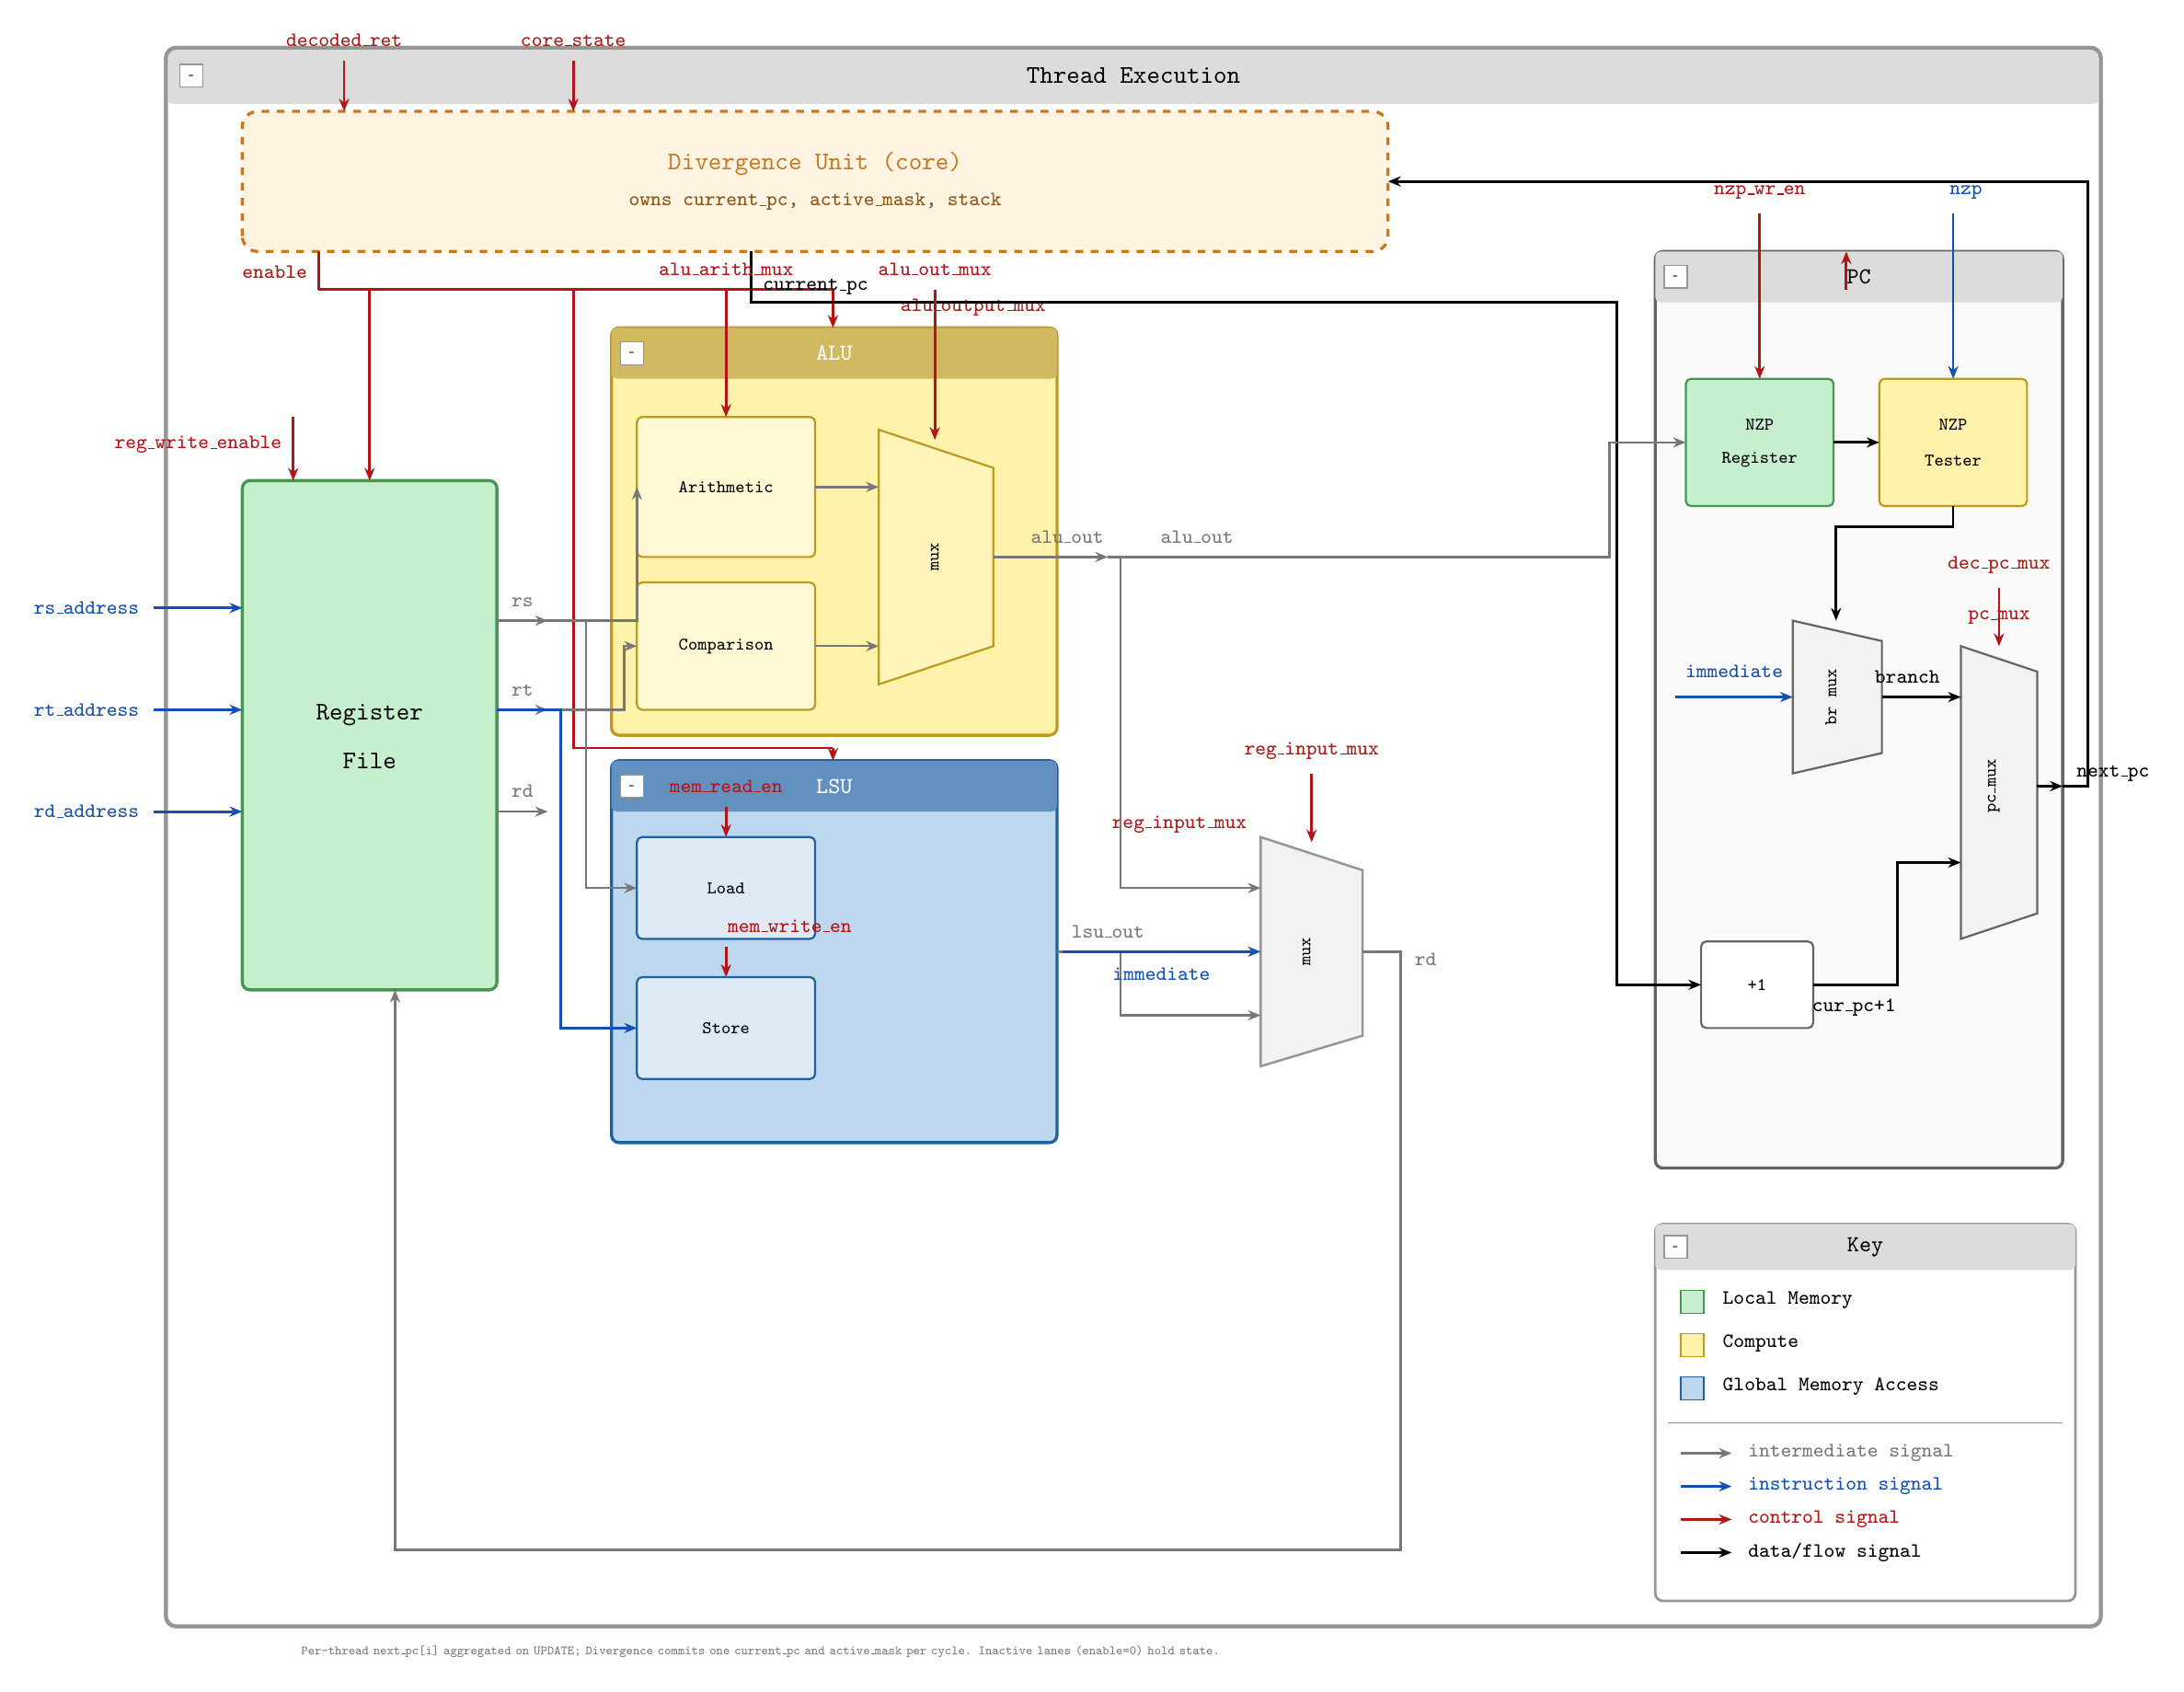
\begin{tikzpicture}[
  font=\small,
  every node/.style={align=center},
  x=1pt, y=1pt
]

%% ════════════════════════════════════════════════════════════════════
%% OUTER BORDER
%% ════════════════════════════════════════════════════════════════════
\def\OX{0} \def\OY{-620} \def\OW{760} \def\OH{620}
\draw[line width=1.5pt, GrayBorder, fill=white, rounded corners=4pt]
  (\OX,\OY) rectangle (\OX+\OW, \OY+\OH);

% Title bar
\fill[TitleBar, rounded corners=3pt]
  (\OX,\OY+\OH-22) rectangle (\OX+\OW,\OY+\OH);
\draw[GrayBorder, line width=1.5pt, rounded corners=4pt]
  (\OX,\OY) rectangle (\OX+\OW,\OY+\OH);
% Title text
\node[font=\normalsize\ttfamily] at (\OX+\OW/2, \OY+\OH-11)
  {Thread Execution};
% Collapse icon
\node[collapseicon] at (\OX+10, \OY+\OH-11) {\tiny{-}};

%% ════════════════════════════════════════════════════════════════════
%% DIVERGENCE UNIT  (top, dashed, orange border)
%% ════════════════════════════════════════════════════════════════════
\def\DX{30} \def\DY{-80} \def\DW{450} \def\DH{55}
\draw[line width=1.2pt, OrangeBorder, dashed, rounded corners=6pt, fill=OrangeFill]
  (\DX,\DY) rectangle (\DX+\DW,\DY+\DH);
\node[font=\normalsize\ttfamily, OrangeBorder] at (\DX+\DW/2, \DY+\DH/2+7)
  {\textbf{Divergence Unit (core)}};
\node[font=\footnotesize\ttfamily, OrangeBorder!70!black] at (\DX+\DW/2, \DY+\DH/2-8)
  {owns current\_pc, active\_mask, stack};

%% ════════════════════════════════════════════════════════════════════
%% REGISTER FILE  (left, green)
%% ════════════════════════════════════════════════════════════════════
\def\RX{30} \def\RY{-370} \def\RW{100} \def\RH{200}
\draw[line width=1.2pt, GreenBorder, fill=GreenFill, rounded corners=3pt]
  (\RX,\RY) rectangle (\RX+\RW,\RY+\RH);
\node[font=\normalsize\ttfamily] at (\RX+\RW/2, \RY+\RH/2+8)
  {Register};
\node[font=\normalsize\ttfamily] at (\RX+\RW/2, \RY+\RH/2-10)
  {File};

%% ════════════════════════════════════════════════════════════════════
%% ALU  (upper-center, yellow)
%% ════════════════════════════════════════════════════════════════════
\def\AX{175} \def\AY{-270} \def\AW{175} \def\AH{160}
\draw[line width=1.2pt, YellowBorder, fill=YellowFill, rounded corners=3pt]
  (\AX,\AY) rectangle (\AX+\AW,\AY+\AH);
% Title bar
\fill[YellowBorder!70!white, rounded corners=2pt]
  (\AX,\AY+\AH-20) rectangle (\AX+\AW,\AY+\AH);
\node[font=\small\ttfamily\bfseries, white] at (\AX+\AW/2, \AY+\AH-10) {ALU};
\node[collapseicon] at (\AX+8,\AY+\AH-10) {\tiny{-}};

% Arithmetic sub-box
\def\ArX{\AX+10} \def\ArY{\AY+70} \def\ArW{70} \def\ArH{55}
\draw[YellowBorder, fill=YellowFill!50!white, line width=0.8pt, rounded corners=2pt]
  (\ArX,\ArY) rectangle (\ArX+\ArW,\ArY+\ArH);
\node[font=\scriptsize\ttfamily] at (\ArX+\ArW/2, \ArY+\ArH/2) {Arithmetic};

% Comparison sub-box
\def\CpX{\AX+10} \def\CpY{\AY+10} \def\CpW{70} \def\CpH{50}
\draw[YellowBorder, fill=YellowFill!50!white, line width=0.8pt, rounded corners=2pt]
  (\CpX,\CpY) rectangle (\CpX+\CpW,\CpY+\CpH);
\node[font=\scriptsize\ttfamily] at (\CpX+\CpW/2, \CpY+\CpH/2) {Comparison};

% alu_output_mux trapezoid (right side of ALU)
% Using a custom shape via coordinates
\def\MuxAX{\AX+105} \def\MuxAY{\AY+20}
\draw[YellowBorder, fill=YellowFill!80!white, line width=0.8pt]
  (\MuxAX,\MuxAY) -- (\MuxAX+45,\MuxAY+15) -- (\MuxAX+45,\MuxAY+85) -- (\MuxAX,\MuxAY+100) -- cycle;
\node[font=\scriptsize\ttfamily, rotate=90] at (\MuxAX+22,\MuxAY+50) {mux};
% label alu_output_mux
\node[lbl_red, anchor=west] at (\MuxAX+5, \AY+\AH+8)
  {alu\_output\_mux};

%% ════════════════════════════════════════════════════════════════════
%% LSU  (lower-center, blue)
%% ════════════════════════════════════════════════════════════════════
\def\LX{175} \def\LY{-430} \def\LW{175} \def\LH{150}
\draw[line width=1.2pt, BlueBorder, fill=BlueFill, rounded corners=3pt]
  (\LX,\LY) rectangle (\LX+\LW,\LY+\LH);
% Title bar
\fill[BlueBorder!70!white, rounded corners=2pt]
  (\LX,\LY+\LH-20) rectangle (\LX+\LW,\LY+\LH);
\node[font=\small\ttfamily\bfseries, white] at (\LX+\LW/2, \LY+\LH-10) {LSU};
\node[collapseicon] at (\LX+8,\LY+\LH-10) {\tiny{-}};

% Load sub-box
\def\LoadX{\LX+10} \def\LoadY{\LY+80} \def\LoadW{70} \def\LoadH{40}
\draw[BlueBorder, fill=BlueFill!50!white, line width=0.8pt, rounded corners=2pt]
  (\LoadX,\LoadY) rectangle (\LoadX+\LoadW,\LoadY+\LoadH);
\node[font=\scriptsize\ttfamily] at (\LoadX+\LoadW/2, \LoadY+\LoadH/2) {Load};

% Store sub-box
\def\StoreX{\LX+10} \def\StoreY{\LY+25} \def\StoreW{70} \def\StoreH{40}
\draw[BlueBorder, fill=BlueFill!50!white, line width=0.8pt, rounded corners=2pt]
  (\StoreX,\StoreY) rectangle (\StoreX+\StoreW,\StoreY+\StoreH);
\node[font=\scriptsize\ttfamily] at (\StoreX+\StoreW/2, \StoreY+\StoreH/2) {Store};

%% ════════════════════════════════════════════════════════════════════
%% reg_input_mux  (center, trapezoid)
%% ════════════════════════════════════════════════════════════════════
\def\RIMX{430} \def\RIMY{-400}
\draw[GrayBorder, fill=GrayFill, line width=0.9pt]
  (\RIMX,\RIMY) -- (\RIMX+40,\RIMY+12) -- (\RIMX+40,\RIMY+77) -- (\RIMX,\RIMY+90) -- cycle;
\node[font=\scriptsize\ttfamily, rotate=90] at (\RIMX+18,\RIMY+45) {mux};
% label
\node[lbl_red, anchor=east] at (\RIMX-2, \RIMY+95)
  {reg\_input\_mux};

%% ════════════════════════════════════════════════════════════════════
%% PC  (upper-right, light gray)
%% ════════════════════════════════════════════════════════════════════
\def\PX{585} \def\PY{-440} \def\PW{160} \def\PH{360}
\draw[line width=1.2pt, PCBorder, fill=PCFill, rounded corners=3pt]
  (\PX,\PY) rectangle (\PX+\PW,\PY+\PH);
% Title bar
\fill[TitleBar, rounded corners=2pt]
  (\PX,\PY+\PH-20) rectangle (\PX+\PW,\PY+\PH);
\node[font=\small\ttfamily, black] at (\PX+\PW/2, \PY+\PH-10) {PC};
\node[collapseicon] at (\PX+8,\PY+\PH-10) {\tiny{-}};

% NZP Register sub-box (green, upper-left)
\def\NZPRX{\PX+12}  \def\NZPRY{\PY+260} \def\NZPRW{58} \def\NZPRH{50}
\draw[GreenBorder, fill=GreenFill, line width=0.8pt, rounded corners=2pt]
  (\NZPRX,\NZPRY) rectangle (\NZPRX+\NZPRW,\NZPRY+\NZPRH);
\node[font=\scriptsize\ttfamily] at (\NZPRX+\NZPRW/2,\NZPRY+\NZPRH/2+7) {NZP};
\node[font=\scriptsize\ttfamily] at (\NZPRX+\NZPRW/2,\NZPRY+\NZPRH/2-7) {Register};

% NZP Tester sub-box (yellow, right of NZP Reg)
\def\NZPTX{\PX+88} \def\NZPTY{\PY+260} \def\NZPTW{58} \def\NZPTH{50}
\draw[YellowBorder, fill=YellowFill, line width=0.8pt, rounded corners=2pt]
  (\NZPTX,\NZPTY) rectangle (\NZPTX+\NZPTW,\NZPTY+\NZPTH);
\node[font=\scriptsize\ttfamily] at (\NZPTX+\NZPTW/2,\NZPTY+\NZPTH/2+7) {NZP};
\node[font=\scriptsize\ttfamily] at (\NZPTX+\NZPTW/2,\NZPTY+\NZPTH/2-7) {Tester};

% +1 box (lower-left)
\def\POX{\PX+18} \def\POY{\PY+55} \def\POW{44} \def\POH{34}
\draw[PCBorder, fill=white, line width=0.8pt, rounded corners=2pt]
  (\POX,\POY) rectangle (\POX+\POW,\POY+\POH);
\node[font=\scriptsize\ttfamily] at (\POX+\POW/2,\POY+\POH/2) {+1};

% branch mux (upper-right trapezoid inside PC)
\def\BRMX{\PX+54} \def\BRMY{\PY+155}
\draw[PCBorder, fill=GrayFill, line width=0.8pt]
  (\BRMX,\BRMY) -- (\BRMX+35,\BRMY+8) -- (\BRMX+35,\BRMY+52) -- (\BRMX,\BRMY+60) -- cycle;
\node[font=\scriptsize\ttfamily, rotate=90] at (\BRMX+15,\BRMY+30) {br mux};

% pc_mux (far right inside PC)
\def\PCMX{\PX+120} \def\PCMY{\PY+90}
\draw[PCBorder, fill=GrayFill, line width=0.8pt]
  (\PCMX,\PCMY) -- (\PCMX+30,\PCMY+10) -- (\PCMX+30,\PCMY+105) -- (\PCMX,\PCMY+115) -- cycle;
\node[font=\scriptsize\ttfamily, rotate=90] at (\PCMX+13,\PCMY+60) {pc\_mux};
% label
\node[lbl_red, anchor=south] at (\PCMX+15,\PCMY+120) {pc\_mux};


%% ════════════════════════════════════════════════════════════════════
%% KEY BOX  (bottom-right)
%% ════════════════════════════════════════════════════════════════════
\def\KX{585} \def\KY{-610} \def\KW{165} \def\KH{148}
\draw[GrayBorder, fill=white, line width=1pt, rounded corners=3pt]
  (\KX,\KY) rectangle (\KX+\KW,\KY+\KH);
% Key title bar
\fill[TitleBar, rounded corners=2pt]
  (\KX,\KY+\KH-18) rectangle (\KX+\KW,\KY+\KH);
\node[font=\small\ttfamily] at (\KX+\KW/2,\KY+\KH-9) {Key};
\node[collapseicon] at (\KX+8,\KY+\KH-9) {\tiny{-}};

% Color squares
\def\SqSz{9}
\def\SqX{\KX+10}
% Green
\fill[GreenFill, draw=GreenBorder, line width=0.5pt]
  (\SqX,\KY+\KH-35) rectangle (\SqX+\SqSz,\KY+\KH-35+\SqSz);
\node[lbl, anchor=west] at (\SqX+\SqSz+4, \KY+\KH-30) {Local Memory};
% Yellow
\fill[YellowFill, draw=YellowBorder, line width=0.5pt]
  (\SqX,\KY+\KH-52) rectangle (\SqX+\SqSz,\KY+\KH-52+\SqSz);
\node[lbl, anchor=west] at (\SqX+\SqSz+4, \KY+\KH-47) {Compute};
% Blue
\fill[BlueFill, draw=BlueBorder, line width=0.5pt]
  (\SqX,\KY+\KH-69) rectangle (\SqX+\SqSz,\KY+\KH-69+\SqSz);
\node[lbl, anchor=west] at (\SqX+\SqSz+4, \KY+\KH-64) {Global Memory Access};

% Divider
\draw[GrayBorder, line width=0.5pt]
  (\KX+5,\KY+\KH-78) -- (\KX+\KW-5,\KY+\KH-78);

% Signal type entries
% Gray hollow arrow
\def\ArrY{\KY+\KH-90}
\draw[arr_gray] (\SqX,\ArrY) -- (\SqX+20,\ArrY);
\node[lbl_gray, anchor=west] at (\SqX+23,\ArrY) {intermediate signal};

\def\ArrY{\KY+\KH-103}
\draw[arr_blue] (\SqX,\ArrY) -- (\SqX+20,\ArrY);
\node[lbl_blue, anchor=west] at (\SqX+23,\ArrY) {instruction signal};

\def\ArrY{\KY+\KH-116}
\draw[arr_red] (\SqX,\ArrY) -- (\SqX+20,\ArrY);
\node[lbl_red, anchor=west] at (\SqX+23,\ArrY) {control signal};

\def\ArrY{\KY+\KH-129}
\draw[arr] (\SqX,\ArrY) -- (\SqX+20,\ArrY);
\node[lbl, anchor=west] at (\SqX+23,\ArrY) {data/flow signal};


%% ════════════════════════════════════════════════════════════════════
%% SIGNALS — Divergence Unit inputs/outputs
%% ════════════════════════════════════════════════════════════════════

% decoded_ret → Divergence (red, from top)
\draw[arr_red] (\DX+40, \DY+\DH+20) -- (\DX+40, \DY+\DH);
\node[lbl_red, anchor=south] at (\DX+40,\DY+\DH+22) {decoded\_ret};

% core_state → Divergence (red, from top)
\draw[arr_red] (\DX+130, \DY+\DH+20) -- (\DX+130, \DY+\DH);
\node[lbl_red, anchor=south] at (\DX+130,\DY+\DH+22) {core\_state};

% enable from Divergence → down to Register File, ALU, LSU, PC (4 branches)
% Main trunk down from Divergence bottom
\draw[SigRed, line width=1pt] (\DX+30, \DY) -- (\DX+30, \DY-15);
\node[lbl_red, anchor=east] at (\DX+29, \DY-8) {enable};
% branch to Register File top
\draw[arr_red] (\DX+30, \DY-15) -- (\RX+50, \DY-15) -- (\RX+50, \RY+\RH);
% branch to ALU top
\draw[arr_red] (\AX+87, \DY-15) -- (\AX+87, \AY+\AH);
\draw[SigRed, line width=1pt] (\DX+30,\DY-15) -- (\AX+87, \DY-15);
% branch to LSU top
\draw[SigRed, line width=1pt] (\DX+30,\DY-15) -- (\LX-15, \DY-15)
  -- (\LX-15, \LY+\LH+5) -- (\LX+87, \LY+\LH+5);
\draw[arr_red] (\LX+87, \LY+\LH+5) -- (\LX+87, \LY+\LH);
% branch to PC top
\draw[arr_red] (\PX+75, \DY-15) -- (\PX+75, \PY+\PH);

% current_pc from Divergence → down to PC (+1 box)
\draw[arr, line width=1pt] (\DX+200, \DY) -- (\DX+200, \DY-20)
  -- (\PX-15, \DY-20) -- (\PX-15, \POY+\POH/2)
  -- (\POX, \POY+\POH/2);
\node[lbl, anchor=west] at (\DX+201, \DY-14) {current\_pc};

% next_pc: from PC mux output → up to Divergence
% pc_mux output exits right edge of PC box
\draw[arr] (\PX+\PW, \PCMY+60) -- (\PX+\PW+10, \PCMY+60)
  -- (\PX+\PW+10, \DY+\DH/2) -- (\DX+\DW, \DY+\DH/2);
\node[lbl, anchor=west] at (\PX+\PW+2, \PCMY+65) {next\_pc};

%% ════════════════════════════════════════════════════════════════════
%% SIGNALS — Register File inputs
%% ════════════════════════════════════════════════════════════════════

% reg_write_enable → Register File top (red)
\draw[arr_red] (\RX+20, \RY+\RH+25) -- (\RX+20, \RY+\RH);
\node[lbl_red, anchor=east] at (\RX+19,\RY+\RH+14) {reg\_write\_enable};

% rs_address (blue, into left edge top)
\draw[arr_blue] (\RX-35, \RY+\RH-50) -- (\RX, \RY+\RH-50);
\node[lbl_blue, anchor=east] at (\RX-37, \RY+\RH-50) {rs\_address};
% rt_address (blue)
\draw[arr_blue] (\RX-35, \RY+\RH-90) -- (\RX, \RY+\RH-90);
\node[lbl_blue, anchor=east] at (\RX-37, \RY+\RH-90) {rt\_address};
% rd_address (blue)
\draw[arr_blue] (\RX-35, \RY+\RH-130) -- (\RX, \RY+\RH-130);
\node[lbl_blue, anchor=east] at (\RX-37, \RY+\RH-130) {rd\_address};

% rs out (gray, right edge upper)
\draw[arr_gray] (\RX+\RW, \RY+\RH-55) -- (\RX+\RW+20, \RY+\RH-55);
\node[lbl_gray, anchor=south] at (\RX+\RW+10, \RY+\RH-53) {rs};
% rt out (gray)
\draw[arr_gray] (\RX+\RW, \RY+\RH-90) -- (\RX+\RW+20, \RY+\RH-90);
\node[lbl_gray, anchor=south] at (\RX+\RW+10, \RY+\RH-88) {rt};
% rd out (gray, lower → to reg_input_mux loop)
\draw[arr_gray] (\RX+\RW, \RY+\RH-130) -- (\RX+\RW+20, \RY+\RH-130);
\node[lbl_gray, anchor=south] at (\RX+\RW+10, \RY+\RH-128) {rd};

%% ════════════════════════════════════════════════════════════════════
%% SIGNALS — Register File ↔ ALU (rs, rt gray)
%% ════════════════════════════════════════════════════════════════════
% rs → ALU Arithmetic and Comparison left
\draw[arr_gray] (\RX+\RW, \RY+\RH-55) -- (\ArX, \RY+\RH-55)
  -- (\ArX, \ArY+\ArH/2);
% rt → ALU Arithmetic and Comparison
\draw[arr_gray] (\RX+\RW, \RY+\RH-90) -- (\AX+5, \RY+\RH-90)
  -- (\AX+5, \CpY+\CpH/2) -- (\CpX, \CpY+\CpH/2);

%% ════════════════════════════════════════════════════════════════════
%% SIGNALS — ALU internal
%% ════════════════════════════════════════════════════════════════════
% Arithmetic → mux
\draw[arr_gray] (\ArX+\ArW, \ArY+\ArH/2) -- (\MuxAX, \ArY+\ArH/2);
% Comparison → mux
\draw[arr_gray] (\CpX+\CpW, \CpY+\CpH/2) -- (\MuxAX, \CpY+\CpH/2);
% alu_arithmetic_mux select into Arithmetic top
\draw[arr_red] (\ArX+\ArW/2, \AY+\AH+15) -- (\ArX+\ArW/2, \ArY+\ArH);
\node[lbl_red, anchor=south] at (\ArX+\ArW/2, \AY+\AH+17) {alu\_arith\_mux};

% alu_output_mux select into mux top
\draw[arr_red] (\MuxAX+22, \AY+\AH+15) -- (\MuxAX+22, \MuxAY+96);
\node[lbl_red, anchor=south] at (\MuxAX+22, \AY+\AH+17) {alu\_out\_mux};

% alu_out exits mux right → out of ALU
\draw[arr_gray] (\MuxAX+45, \MuxAY+50) -- (\AX+\AW+20, \MuxAY+50);
\node[lbl_gray, anchor=south] at (\AX+\AW+4, \MuxAY+52) {alu\_out};

%% ════════════════════════════════════════════════════════════════════
%% SIGNALS — ALU → reg_input_mux & PC
%% ════════════════════════════════════════════════════════════════════
% alu_out → reg_input_mux
\draw[arr_gray] (\AX+\AW+20, \MuxAY+50) -- (\AX+\AW+25, \MuxAY+50)
  -- (\AX+\AW+25, \RIMY+70) -- (\RIMX, \RIMY+70);
% alu_out → PC NZP Register
\draw[arr_gray] (\AX+\AW+20, \MuxAY+50) -- (\PX-18, \MuxAY+50)
  -- (\PX-18, \NZPRY+\NZPRH/2) -- (\NZPRX, \NZPRY+\NZPRH/2);
\node[lbl_gray, anchor=south] at (\AX+\AW+55, \MuxAY+52) {alu\_out};

%% ════════════════════════════════════════════════════════════════════
%% SIGNALS — LSU inputs/outputs
%% ════════════════════════════════════════════════════════════════════
% mem_read_enable → Load
\draw[arr_red] (\LoadX+\LoadW/2, \LoadY+\LoadH+12) -- (\LoadX+\LoadW/2, \LoadY+\LoadH);
\node[lbl_red, anchor=south] at (\LoadX+\LoadW/2, \LoadY+\LoadH+14) {mem\_read\_en};

% mem_write_enable → Store
\draw[arr_red] (\StoreX+\StoreW/2, \StoreY+\StoreH+12)
  -- (\StoreX+\StoreW/2, \StoreY+\StoreH);
\node[lbl_red, anchor=south] at (\StoreX+\StoreW/2+25, \StoreY+\StoreH+14) {mem\_write\_en};

% rs → LSU Load (gray)
\draw[arr_gray] (\RX+\RW, \RY+\RH-55) -- (\LX-10, \RY+\RH-55)
  -- (\LX-10, \LoadY+\LoadH/2) -- (\LoadX, \LoadY+\LoadH/2);

% rt → LSU Store (blue — store data)
\draw[arr_blue] (\RX+\RW, \RY+\RH-90) -- (\LX-20, \RY+\RH-90)
  -- (\LX-20, \StoreY+\StoreH/2) -- (\StoreX, \StoreY+\StoreH/2);

% lsu_out → reg_input_mux (gray)
\draw[arr_gray] (\LX+\LW, \LY+\LH/2) -- (\LX+\LW+25, \LY+\LH/2)
  -- (\LX+\LW+25, \RIMY+20) -- (\RIMX, \RIMY+20);
\node[lbl_gray, anchor=south] at (\LX+\LW+20, \LY+\LH/2+2) {lsu\_out};

%% ════════════════════════════════════════════════════════════════════
%% SIGNALS — immediate (blue instruction, local mux inputs)
%% ════════════════════════════════════════════════════════════════════
\draw[arr_blue] (\RIMX-78, \RIMY+45) -- (\RIMX, \RIMY+45);
\node[lbl_blue, anchor=north] at (\RIMX-39, \RIMY+42) {immediate};

% immediate also goes to PC branch mux
\draw[arr_blue] (\PX+8, \BRMY+30) -- (\BRMX, \BRMY+30);
\node[lbl_blue, anchor=south] at (\PX+31, \BRMY+34) {immediate};

%% ════════════════════════════════════════════════════════════════════
%% SIGNALS — reg_input_mux → Register File write-back
%% ════════════════════════════════════════════════════════════════════
% rd output from mux right → loop down → Register File bottom
\draw[arr_gray] (\RIMX+40, \RIMY+45) -- (\RIMX+55, \RIMY+45)
  -- (\RIMX+55, \OY+30)
  -- (\RX+60, \OY+30)
  -- (\RX+60, \RY);
\node[lbl_gray, anchor=west] at (\RIMX+57,\RIMY+42) {rd};

% reg_input_mux select into mux top
\draw[arr_red] (\RIMX+20, \RIMY+115) -- (\RIMX+20, \RIMY+88);
\node[lbl_red, anchor=south] at (\RIMX+20, \RIMY+117) {reg\_input\_mux};

%% ════════════════════════════════════════════════════════════════════
%% SIGNALS — PC internal
%% ════════════════════════════════════════════════════════════════════
% nzp_write_enable → NZP Register top (red)
\draw[arr_red] (\NZPRX+\NZPRW/2, \PY+\PH+15) -- (\NZPRX+\NZPRW/2, \NZPRY+\NZPRH);
\node[lbl_red, anchor=south] at (\NZPRX+\NZPRW/2, \PY+\PH+17) {nzp\_wr\_en};

% nzp (blue) → NZP Tester top
\draw[arr_blue] (\NZPTX+\NZPTW/2, \PY+\PH+15) -- (\NZPTX+\NZPTW/2, \NZPTY+\NZPTH);
\node[lbl_blue, anchor=south] at (\NZPTX+\NZPTW/2+5, \PY+\PH+17) {nzp};

% NZP Register → NZP Tester (black)
\draw[arr] (\NZPRX+\NZPRW, \NZPRY+\NZPRH/2) -- (\NZPTX, \NZPTY+\NZPTH/2);

% NZP Tester → branch mux select (control, into mux top)
\draw[arr] (\NZPTX+\NZPTW/2, \NZPTY)
  -- (\NZPTX+\NZPTW/2, \NZPTY-8)
  -- (\BRMX+17, \NZPTY-8)
  -- (\BRMX+17, \BRMY+60);

% +1 output → pc_mux lower input (black)
\draw[arr] (\POX+\POW, \POY+\POH/2) -- (\PCMX-25, \POY+\POH/2)
  -- (\PCMX-25, \PCMY+30) -- (\PCMX, \PCMY+30);
\node[lbl, anchor=north] at (\POX+\POW+16, \POY+\POH/2-2) {cur\_pc+1};

% branch mux output → pc_mux upper input (black)
\draw[arr] (\BRMX+35, \BRMY+30) -- (\PCMX, \BRMY+30);
\node[lbl, anchor=south] at (\BRMX+45, \BRMY+32) {branch};

% pc_mux select (decoded_pc_mux, red into top)
\draw[arr_red] (\PCMX+15, \PCMY+138) -- (\PCMX+15, \PCMY+115);
\node[lbl_red, anchor=south] at (\PCMX+15, \PCMY+140) {dec\_pc\_mux};

% next_pc exits PC right → routed up to Divergence
\draw[arr] (\PCMX+30, \PCMY+60) -- (\PX+\PW, \PCMY+60);
% (already drawn above as part of next_pc → Divergence path)


%% ════════════════════════════════════════════════════════════════════
%% FOOTNOTE
%% ════════════════════════════════════════════════════════════════════
\node[font=\tiny\ttfamily, SigGray, anchor=north west, text width=450pt] 
  at (\OX+5, \OY-4)
  {Per-thread next\_pc[i] aggregated on UPDATE; Divergence commits one current\_pc and active\_mask per cycle. Inactive lanes (enable=0) hold state.};

\end{tikzpicture}
\end{document}